\documentclass[11pt]{article}

\usepackage[a4paper,margin=2.4cm]{geometry}
\usepackage{amsmath,amssymb}
\usepackage{graphicx}
\usepackage{booktabs}
\usepackage{xcolor}
\usepackage{tikz}
\usetikzlibrary{arrows.meta,positioning,fit,backgrounds,calc}
\usepackage[font=small,labelfont=bf]{caption}
\usepackage{float}
\usepackage{enumitem}
\usepackage{microtype}
\usepackage[hidelinks]{hyperref}

% ---- lensing brand palette (DESIGN.md) ----
\definecolor{lensorange}{HTML}{D98A00}
\definecolor{lensorangeb}{HTML}{F59E0B}
\definecolor{lensslate}{HTML}{3A3A42}
\definecolor{lensblue}{HTML}{4F7BF6}
\definecolor{lensgrey}{HTML}{6B6878}
\definecolor{lenspaper}{HTML}{F9F9FA}

\hypersetup{colorlinks=true,linkcolor=lensslate,urlcolor=lensblue,citecolor=lensblue}
\setlength{\parindent}{0pt}
\setlength{\parskip}{0.55em}

\newcommand{\file}[1]{\texttt{\small #1}}
\newcommand{\code}[1]{\texttt{\small #1}}

% callout box for documented-vs-inferred provenance
\newcommand{\note}[2]{%
  \begin{center}\small
  \fcolorbox{lensslate}{lenspaper}{\parbox{0.95\linewidth}{%
  \textbf{\color{lensslate}#1.}\ #2}}\end{center}}

\title{\vspace{-1.4cm}
  
\includegraphics[height=1.25cm]{assets/lensing-logo.pdf}\\[0.7em]
  \textbf{The Models of Pathfinder}\\[0.2em]
  {\large Architecture, Training, and Algorithmics of a\\ Serverless Music-Journey Engine}}
\author{\textsc{lensing}\,\,$\cdot$\,\,spotify-pathfinder\\
  \small\texttt{spotify-predict-engagement} $\rightarrow$ \texttt{app} (Cloudflare Worker + WASM)}
\date{June 2026}

\begin{document}
\maketitle

\begin{abstract}\noindent
\emph{Pathfinder} renders a ``musical journey'' between two Spotify tracks: an A\textsuperscript{*}
search threads a path through a 23{,}529-track map of listening taste, drawn in 3D. The system is
unusual in that it runs \emph{entirely} on a single Cloudflare Worker --- no Python origin, no
vector database at request time --- by compiling all numeric work to WebAssembly and baking a
static snapshot of every model's \emph{output} into the deployed artifact. This report documents
the seven models and algorithms behind it: a song autoencoder that defines the taste map, a
gradient-boosted classifier that scores track ``fit'', a distilled cold-start projector, a
satisfaction-weighted transition model, a symmetric $k$-NN graph, the A\textsuperscript{*}{+}densify
pathfinder, and a power-iteration PCA for the 3D view. For each we give structure, the training
recipe, and the design rationale --- grounding every claim in the \texttt{lensing} training project
and clearly flagging what is documented versus inferred. We include error surfaces from real
parameter sweeps: a freshly-run hyperparameter scan of the rotation classifier on its true champion
dataset, and response surfaces of the A\textsuperscript{*} cost weights over the real corpus.
\end{abstract}

%====================================================================
\section{System overview: the lensing platform}
\label{sec:overview}

The models were produced by \textbf{lensing}, a prediction-lab framework that ``shapes itself around
your dataset the way mass bends light'': point it at a Qdrant corpus, declare a target and fields in
\file{domain.toml}, and it bakes datasets, trains a registry of candidate predictors, and promotes
the best to a named export. The Pathfinder \file{app} is the serverless \emph{inference} instance of
one such lensing problem (\file{spotify-predict-engagement}).

The defining architectural split is \textbf{train offline, infer at the edge}
(Figure~\ref{fig:pipeline}). Every learned model runs once, offline, over the corpus; its outputs
--- 64-d latent vectors, per-track fit scores, transition tables, the $k$-NN graph --- are written
to binary snapshot files (\file{corpus.bin}, \file{transitions.json}, \file{projector.bin}). At
request time the Rust/WASM core reads those frozen outputs and does \emph{pure arithmetic}: search,
densify, PCA. An in-corpus $\rightarrow$ in-corpus route touches \emph{zero} live model inference.
Only off-map (cold-start) tracks invoke a model at request time --- a text embedding plus the
projector --- because the geometry for arbitrary tracks cannot be precomputed.

\note{Why this shape}{The Workers Free plan caps each request at ${\sim}10$\,ms of CPU. Live
gradient-boosting or neural inference over 23k tracks cannot fit; precomputing every model output
and shipping it as a memory-mapped snapshot does. The cost is staleness: refreshing the corpus means
re-running the offline build and redeploying.}

\begin{figure}[H]\centering
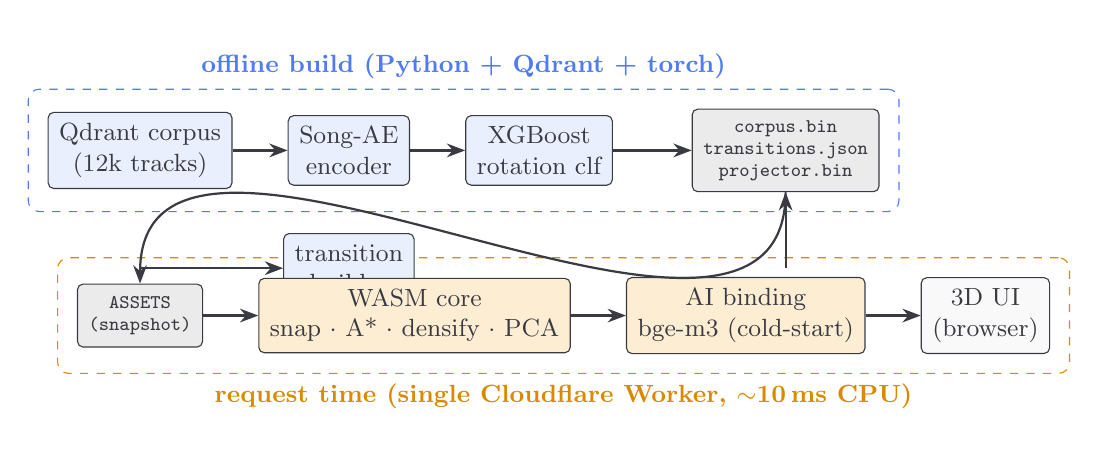
\begin{tikzpicture}[
  font=\small,
  box/.style={draw=lensslate,rounded corners=2pt,align=center,inner sep=4pt,minimum height=8mm},
  off/.style={box,fill=lensblue!12},
  on/.style={box,fill=lensorangeb!18},
  art/.style={box,fill=lensslate!10,font=\ttfamily\scriptsize},
  ar/.style={-{Stealth[]},lensslate,thick}, every node/.style={text=lensslate}]
  % offline
  \node[off] (qd) {Qdrant corpus\\(12k tracks)};
  \node[off,right=7mm of qd] (ae) {Song-AE\\encoder};
  \node[off,right=7mm of ae] (xgb) {XGBoost\\rotation clf};
  \node[off,below=6mm of ae] (tr) {transition\\builder};
  \node[art,right=10mm of xgb] (snap) {corpus.bin\\transitions.json\\projector.bin};
  \draw[ar] (qd)--(ae); \draw[ar] (ae)--(xgb); \draw[ar] (qd|-tr)--(tr);
  \draw[ar] (xgb)--(snap); \draw[ar] (tr-|snap)--(snap);
  % request-time
  \node[art,below=12mm of qd] (asset) {ASSETS\\(snapshot)};
  \node[on,right=7mm of asset] (wasm) {WASM core\\snap $\cdot$ A* $\cdot$ densify $\cdot$ PCA};
  \node[on,right=7mm of wasm] (ai) {AI binding\\bge-m3 (cold-start)};
  \node[box,fill=lenspaper,right=7mm of ai] (ui) {3D UI\\(browser)};
  \draw[ar] (asset)--(wasm); \draw[ar] (wasm)--(ai); \draw[ar] (ai)--(ui);
  \draw[ar] (snap) to[out=-90,in=90] (asset);
  \begin{scope}[on background layer]
    \node[draw=lensblue,dashed,rounded corners,fit=(qd)(snap),inner sep=7pt,label={[lensblue]above:\textbf{offline build (Python + Qdrant + torch)}}]{};
    \node[draw=lensorange,dashed,rounded corners,fit=(asset)(ui),inner sep=7pt,label={[lensorange]below:\textbf{request time (single Cloudflare Worker, ${\sim}$10\,ms CPU)}}]{};
  \end{scope}
\end{tikzpicture}
\caption{The train-offline / infer-at-the-edge split. Learned models (blue) run once; the Worker
(orange) reads their frozen outputs and does only arithmetic, except for the cold-start embedding.}
\label{fig:pipeline}
\end{figure}

Table~\ref{tab:models} summarizes the seven components. The rest of the paper takes them in turn.

\begin{table}[H]\centering\small
\caption{The seven models / algorithms. ``Runs'' is when inference happens.}
\label{tab:models}
\begin{tabular}{@{}llll@{}}
\toprule
Component & Type & In $\rightarrow$ Out & Runs \\
\midrule
Song-AE & autoencoder (MLP) & 539 $\rightarrow$ 64 & offline (defines the map) \\
XGBoost rotation clf & gradient-boosted trees & 115 $\rightarrow$ 1 & offline (bakes \code{fit}) \\
Cold-start projector & MLP (distilled) & 1179 $\rightarrow$ 64 & request (off-map only) \\
Transition model & weighted bigram + back-off & meta $\rightarrow$ affinity & request (in WASM) \\
$k$-NN graph & symmetric cosine, $k{=}20$ & --- & offline (baked edges) \\
A\textsuperscript{*}{+}densify & heuristic graph search & graph $\rightarrow$ path & request (in WASM) \\
PCA & power iteration {+} deflation & 64 $\rightarrow$ 3 & request (per route) \\
\bottomrule
\end{tabular}
\end{table}

%====================================================================
\section{The taste map: the Song autoencoder}
\label{sec:songae}

\textbf{Role.} The Song-AE's 64-dimensional latent \emph{is} the coordinate system everything else
lives in. Cosine distance between two latents is the system's notion of musical distance; the $k$-NN
graph, the A\textsuperscript{*} heuristic, and the 3D PCA all operate on these vectors. They are
L2-normalized, so $\cos$ similarity reduces to a dot product.

\textbf{Structure} (\file{pipeline/build\_song\_ae.py}). A symmetric undercomplete autoencoder:
\[
\text{enc}:\ \mathbb{R}^{539}\xrightarrow{\;W_1\;}\mathbb{R}^{256}\xrightarrow{\text{ReLU}}
\xrightarrow{\;W_2\;}\mathbb{R}^{64},\qquad
\text{dec}:\ \mathbb{R}^{64}\rightarrow\mathbb{R}^{256}\xrightarrow{\text{ReLU}}\mathbb{R}^{539}.
\]
The 539-d input concatenates five blocks of heterogeneous evidence about a track
(Figure~\ref{fig:blocks}, left): a 384-d multilingual text embedding
(\code{paraphrase-multilingual-MiniLM-L12-v2}) of a natural-language ``content document'';
10 z-scored numerics (popularity, followers and duration via $\log 1p$, release year, $\dots$);
22 acoustic dims (11 ReccoBeats audio features {+} 11 missing-flags, \S\ref{sec:coldstart}); a
120-way genre multi-hot; and a 3-way album-type one-hot.

\textbf{Training.} Block-wise mean-squared reconstruction, summed with equal weight per modality so a
large block (text) cannot dominate a small one (album):
\[
\mathcal{L} \;=\; \sum_{b\in\text{blocks}} \big\lVert \hat{x}_{[b]} - x_{[b]} \big\rVert_2^2 .
\]
Adam ($\text{lr}=10^{-3}$, weight decay $10^{-5}$), batch 256, 200 epochs, seed 42, all 12{,}256
tracks (no held-out split --- the goal is a faithful corpus embedding, not generalization to unseen
tracks). The encoder weights are frozen into \file{song\_ae.pt}; the deployed corpus latents are its
outputs.

\begin{figure}[H]\centering
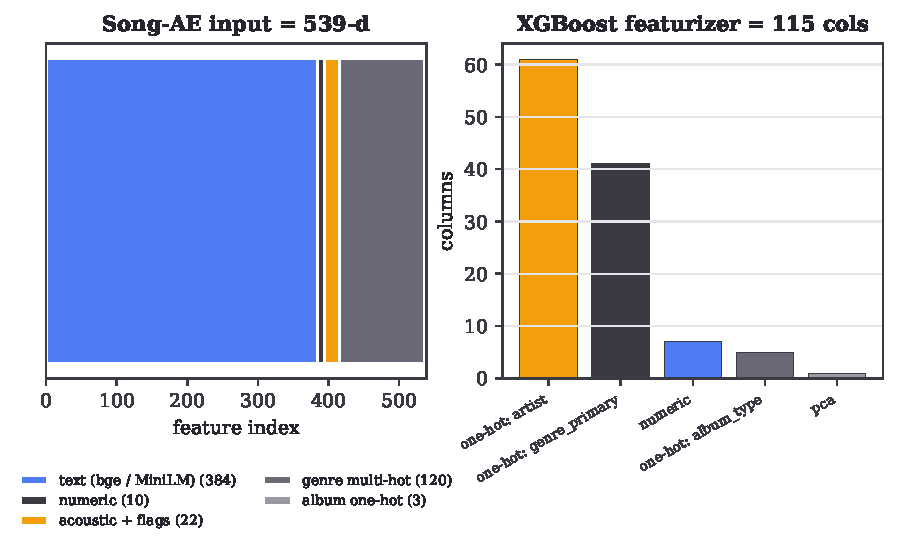
\includegraphics[width=\linewidth]{figures/fig_feature_blocks.pdf}
\caption{Left: the 539-d Song-AE input as five concatenated modality blocks. Right: the
\emph{separate} 115-column featurizer the XGBoost classifier actually uses --- dominated by identity
one-hots (artist, genre), not dense vectors (\S\ref{sec:identity}).}
\label{fig:blocks}
\end{figure}

\note{Documented}{Architecture, loss, and optimizer are read directly from
\file{pipeline/build\_song\_ae.py}. \textit{Not} documented: why 64 latent dims specifically, or a
study of deeper encoders --- the latent width is a fixed constant across the system.}

%====================================================================
\section{Engagement / fit: the XGBoost rotation classifier}
\label{sec:xgb}

\textbf{What it predicts.} Each track gets a scalar \code{fit} $\in[0,1]$ used by A\textsuperscript{*}
to prefer ``sticky'' tracks. \code{fit} is \emph{not} a regression of play-count; it is the
calibrated probability of \textbf{rotation}, the binary target \code{rotation = (play\_count $\ge$ 2)}
--- ``did the listener come back to this track?'' (\file{domain.toml}). The model is an XGBoost
binary classifier (\code{objective=binary:logistic}); its positive-class probability is exported to
ONNX and, at snapshot-build time, scored over the whole corpus, min--max normalized, and written as
the \code{fit} column of \file{corpus.bin}.

\textbf{Why rotation, not engagement.} The project originally targeted
\code{engagement = play\_count $\times$ completion\_ratio} ($\log 1p$). It pivoted to rotation because
the binary taste-fit signal is more learnable (AUC ${\sim}0.73$--$0.77$) and spreads naturally into a
$[0,1]$ fit weight (\file{PROJECT-FACTS.md}). The shipped champion scores \textbf{AUC 0.7429},
logloss 0.5883, accuracy 0.6846 on a 2{,}451-track held-out split.

\textbf{Features.} A \emph{frozen} 115-column featurizer (Figure~\ref{fig:blocks}, right), distinct
from the Song-AE's 539-d input: 1 PCA floor component of the latent, a handful of numerics, and
$\sim$107 one-hot columns for \code{artist}, \code{genre\_primary}, and \code{album\_type} (each with
an \code{\_\_other\_\_} catch-all). Hyperparameters (\file{predictors/xgboost-classifier/train.py}):
500 trees, \code{max\_depth} 6, \code{learning\_rate} 0.05, \code{subsample}/\code{colsample\_bytree}
0.8, \code{reg\_lambda} 1.0, seed 42.

\begin{figure}[H]\centering
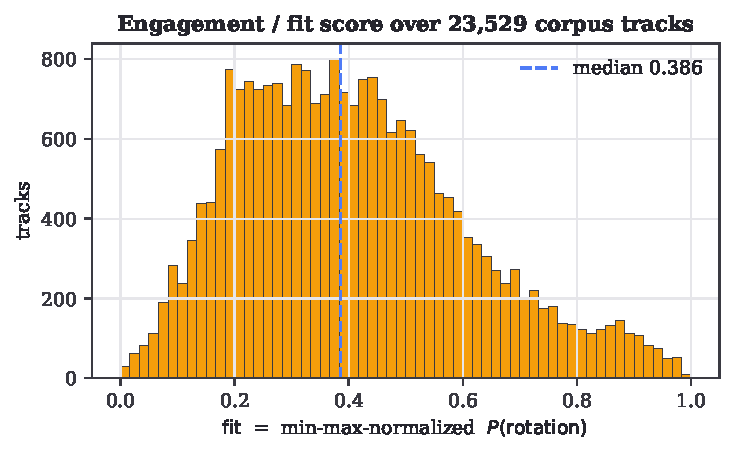
\includegraphics[width=0.62\linewidth]{figures/fig_fit_hist.pdf}
\caption{The \code{fit} column actually shipped in \file{corpus.bin}: the min--max-normalized
rotation probability for all 23{,}529 corpus tracks. A\textsuperscript{*} pays
$W_{\text{FIT}}(1-\code{fit})$ per hop (\S\ref{sec:astar}).}
\label{fig:fithist}
\end{figure}

\subsection{An error hypersurface: the deferred hyperparameter scan}
\label{sec:xgbsweep}

The champion's hyperparameters are sensible defaults, \emph{not} the result of a grid search.
\file{PROJECT-FACTS.md} explicitly names ``a depth\,/\,n\_estimators\,/\,learning\_rate scan'' as
``the next real lever for AUC'' and \emph{defers} it. We ran that deferred scan for this report,
directly on the real champion dataset \file{ds-20260609-141622-p1-s42} and frozen split, using the
exact reference training path (\code{XGBClassifier}, AUC on positive-class probability). Our harness
reproduces the published 0.7429 to four decimals before sweeping, so the surface is trustworthy.

\begin{figure}[H]\centering
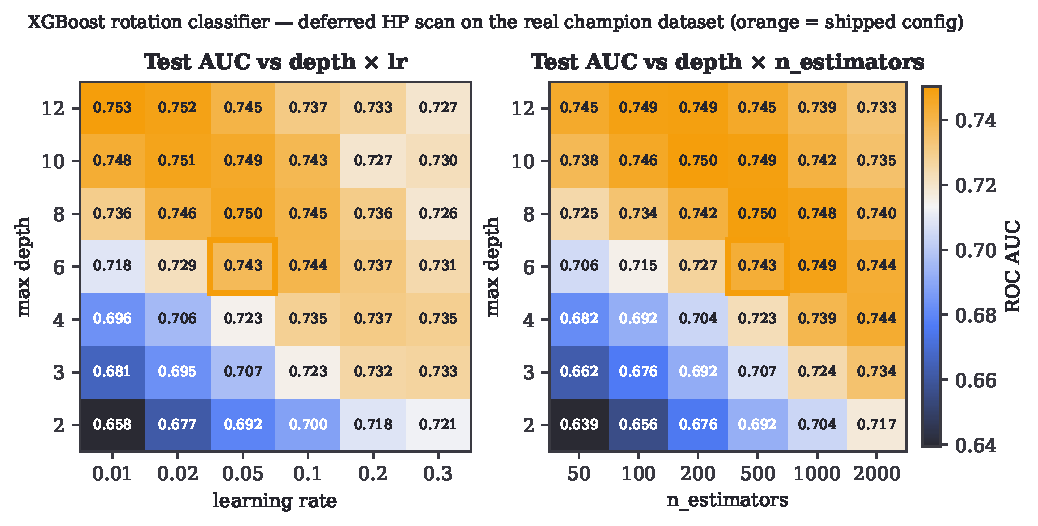
\includegraphics[width=\linewidth]{figures/fig_xgb_sweep.pdf}
\caption{\textbf{Test-AUC error surfaces from the deferred scan} (real data, computed for this
report). Left: \code{max\_depth} $\times$ \code{learning\_rate}; right: \code{max\_depth} $\times$
\code{n\_estimators}. The orange cell is the shipped config. The classic boosting ridge is visible
(low lr wants more depth/trees). Best cell: AUC \textbf{0.7534} at depth 12, lr 0.01 --- only
$+0.011$ over the champion, \emph{inside} the measured $2\sigma=0.0126$ noise band
(\S\ref{sec:identity}). The scan was reasonably deferred: no cell is a significant win.}
\label{fig:xgbsweep}
\end{figure}

\note{Provenance}{The numbers in Figure~\ref{fig:xgbsweep} are genuine --- 84 XGBoost fits on the
real frozen split (\file{docs/sweeps/run\_xgb\_sweep.py}). They are \emph{new} work, not a recovered
training log, because no such grid was ever stored. The takeaway is honest: tuning moves AUC less
than seed noise.}

%====================================================================
\section{Why identity beats dense vectors (the central lesson)}
\label{sec:identity}

The most strongly documented finding of the whole project is a negative one about features. Across
two targets and six confirmations, \textbf{artist/genre identity one-hots exploited by trees beat
every dense representation}: the co-listening embedding, the 384-d content-text embedding, the 11
acoustic features, and --- notably --- the Song-AE's own 64-d latent all \emph{hurt or diluted} the
score. ``The taste-fit signal is predicted by artist/genre \textsc{identity}\,$\dots$\,not by
descriptive attributes nor by distance/margin models'' (\file{PROJECT-FACTS.md}).

\begin{figure}[H]\centering
\begin{minipage}[t]{0.6\linewidth}\centering
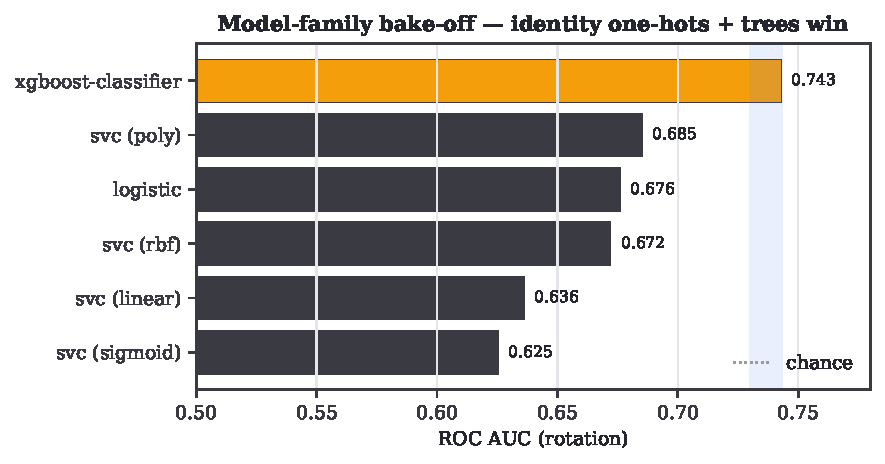
\includegraphics[width=\linewidth]{figures/fig_bakeoff.pdf}
\end{minipage}\hfill
\begin{minipage}[t]{0.38\linewidth}\centering
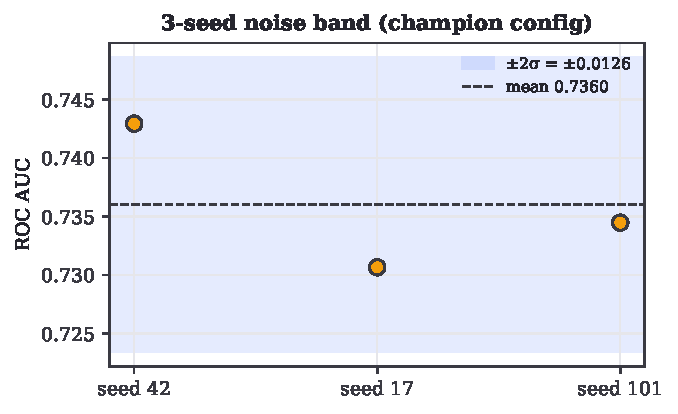
\includegraphics[width=\linewidth]{figures/fig_noiseband.pdf}\\[0.4em]
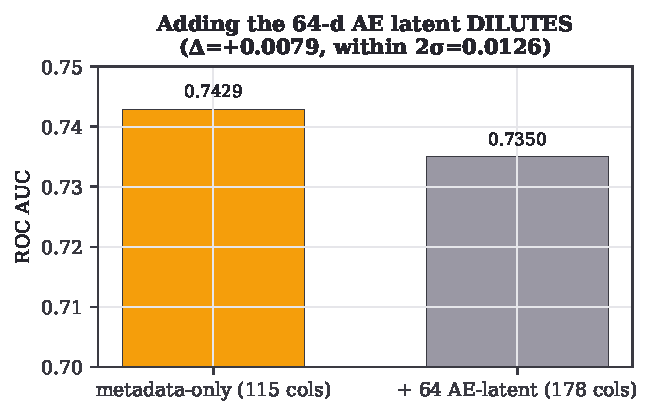
\includegraphics[width=\linewidth]{figures/fig_variants.pdf}
\end{minipage}
\caption{Real logged runs on the rotation champion dataset. \textbf{Left:} family bake-off --- the
tree beats every dense distance/margin model (SVC kernels, logistic) by 4.6--9.3 noise bands.
\textbf{Top-right:} the 3-seed noise band that calibrates significance ($\sigma_{\text{AUC}}=0.0063$).
\textbf{Bottom-right:} adding the 64-d AE latent as features \emph{dilutes} AUC by $0.0079$.}
\label{fig:bakeoff}
\end{figure}

This is why the Song-AE latent and the fit-prediction featurizer are \emph{deliberately separate}
(Figure~\ref{fig:blocks}): the latent is excellent as a \emph{geometry} for the map (it places
similar tracks near each other) yet a poor \emph{feature} for predicting rotation, where raw identity
carries the signal. A meta-lesson the project states plainly: ``features usually beat architecture;
scan dataset-level axes before deep hyperparameter scans'' --- consistent with the flat surface in
Figure~\ref{fig:xgbsweep}.

\note{Pitfalls documented}{The project records concrete traps: SVR with an $\varepsilon$-tube on a
\{0,1\} target posts a deceptively low MAE while being worse-than-mean on $R^2$; MAE-tuned blends
collapse their weight onto that artifact ($w\to0$). These motivated switching to AUC/logloss as the
honest classification metrics.}

%====================================================================
\section{Cold-start: projecting an off-map track}
\label{sec:coldstart}

When a requested track is not in the corpus, it must be placed in the 64-d latent space at request
time. Two instances solve this differently:

\begin{itemize}[leftmargin=1.4em,itemsep=2pt]
\item \textbf{Reference} (\file{pipeline/predict\_spotify\_url.py}): run the \emph{actual} frozen
Song-AE encoder, then the dataset's frozen PCA basis. Needs torch + sentence-transformers.
\item \textbf{App} (\file{worker-core/src/project.rs}, built by \file{tools/build\_snapshot.py}): a
Worker cannot run torch, so the app ships a \textbf{distilled projector} --- a small MLP
$\mathbb{R}^{1179}\!\to\!256\!\to\!64$ trained to \emph{reproduce} the corpus Song-AE latents from
features obtainable live (a 1024-d \code{bge-m3} embedding from the Workers AI binding, plus the same
numeric/acoustic/genre/album blocks). Loss is cosine distance to the L2-normalized target latent;
Adam $10^{-3}$, batch 512, 120 epochs; validated by self-recall@1.
\end{itemize}

Both land the track in the same space, after which it \emph{snaps} to the nearest corpus anchor and
routing proceeds. The projector is a lossy \emph{translator} from ``features available in the
Worker'' to ``the Song-AE representation'', which is why the app then trusts the nearest real anchor
over the raw projected point.

\begin{figure}[H]\centering
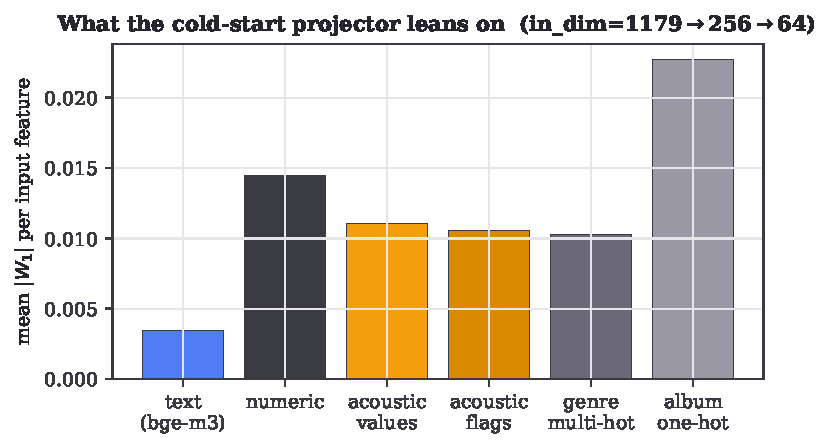
\includegraphics[width=0.66\linewidth]{figures/fig_projector_blocks.pdf}
\caption{Mean $|W_1|$ per input feature in the deployed projector (\file{projector.bin}), by input
block. The text embedding and numerics carry most of the first-layer weight; acoustic
\emph{missing-flags} carry real signal too (below).}
\label{fig:projblocks}
\end{figure}

\textbf{The missing-flag block.} Acoustic features are often absent. Imputing the mean is fine, but
because features are z-scored, an imputed value becomes exactly $0$ --- \emph{indistinguishable from a
genuinely average track}. Each acoustic feature therefore contributes \emph{two} inputs: a value and
a 0/1 ``was-this-real'' flag (laid out as two contiguous blocks, matching the trained weight order):

\begin{table}[H]\centering\small
\caption{Mean-imputation made honest. Rows 2--4 all yield value $0.0$ for different reasons; the flag
disambiguates ``placeholder'' from ``genuinely average''.}
\label{tab:flag}
\begin{tabular}{@{}lcccc@{}}
\toprule
feature & raw & stats $(\mu,\sigma)$ & value slot $=(x-\mu)/\sigma$ & flag \\
\midrule
danceability & 0.8 & (0.6,\,0.2) & $+1.0$ & 0 \\
energy & --- (missing) & (0.65,\,0.15) & $0.0$ \emph{(imputed)} & \textbf{1} \\
valence & 0.5 & (0.5,\,0.2) & $0.0$ \emph{(real)} & 0 \\
tempo & 120 & (120,\,30) & $0.0$ \emph{(real)} & 0 \\
\bottomrule
\end{tabular}
\end{table}

%====================================================================
\section{The transition model: what naturally follows what}
\label{sec:transit}

A\textsuperscript{*} does not move on geometry alone; it also prefers transitions that real listening
sessions actually make. The transition model (\file{pipeline/corpus/transitions.py}, ported to
\file{worker-core/src/transit.rs}) is built from a sessionized play log. Consecutive non-skip plays
($\ge 30$\,s) form a \textbf{track bigram}, each edge weighted by the destination's
\emph{satisfaction} (e.g. \code{trackdone}=1.0, \code{fwdbtn}=0.25). Bigrams are aggregated up to
artist$\to$artist and genre$\to$genre conditionals.

\textbf{Affinity with back-off.} Track-level data is sparse --- most tracks have only a handful of
recorded successors --- so the next-track affinity blends the track-specific bigram with a coarser
artist/genre estimate, trusting the bigram only as far as its evidence goes:
\[
\text{aff}(u,v) = \tau\,P(v\mid u) + (1-\tau)\underbrace{\big[\,0.6\,P_{\text{art}} + 0.4\,P_{\text{gen}}\big]}_{\text{back-off prior}},
\qquad \tau = \frac{n_u}{n_u + K},\ \ K=8 .
\]
The \emph{support} $n_u$ is what drives $\tau$: it is the total number of times track $u$ was
followed by a kept (non-skip) track anywhere in the log --- the amount of evidence behind
$P(v\mid u)$. The trust weight $\tau\in[0,1)$ is just that evidence divided by itself plus a constant
$K$, where $K$ acts as a \emph{pseudo-count} --- as if we had pre-seen $K$ plays that vote for the
back-off prior. In words, $\tau = $ ``real observations $/$ (real $+$ $K$ imaginary) observations'':
\[
n_u=0\ \Rightarrow\ \tau=0\ \text{(pure back-off)},\quad
n_u=K=8\ \Rightarrow\ \tau=0.5\ \text{(half each)},\quad
n_u=40\ \Rightarrow\ \tau\approx0.83\ \text{(mostly bigram)}.
\]
So a track seen only a few times leans on its artist/genre statistics, while a heavily-observed
track trusts its own successors; $K=8$ is the crossover support at which the two carry equal weight
(Figure~\ref{fig:transit}).

\textbf{Context: what a ``lift'' is.} Listening also has a rhythm --- some genres belong to the
evening, some to a shuffle session --- and the model captures this with \emph{lifts}. A lift is just
a multiplier that says how much more (or less) a genre is played in a given context than it is
overall:
\[
\text{lift}(g\mid c)\;=\;\frac{P(g\mid c)}{P(g)}
\;=\;\frac{\text{rate of genre } g \text{ within context } c}{\text{rate of } g \text{ across the whole log}} .
\]
So $\text{lift}=1$ is neutral (the context makes no difference), $\text{lift}>1$ \emph{boosts} the
genre (it is over-represented there), and $\text{lift}<1$ \emph{suppresses} it. If jazz plays twice
as often in the evening as it does on average, its evening lift is $2$.

A candidate track $v$ collects the product of three such lifts --- its genre under the current
time-of-day, its genre under shuffle-vs-linear, and (for sufficiently popular tracks) the track
itself under the time-of-day:
\[
\text{ctx}(v)=\text{lift}_{\text{tod}}(g_v)\cdot\text{lift}_{\text{shuf}}(g_v)\cdot\text{lift}_{\text{tod}}(v).
\]
Two guards keep these honest: each lift is \emph{shrunk toward $1$} in proportion to how little data
supports it (a genre seen only a few times in a context stays near neutral instead of swinging to an
extreme), and the product is \emph{clipped to} $[0.2,5]$ so no single context can dominate. This
$\text{ctx}(v)$ is exactly what \code{context\_fit} returns; like the affinity above, it is min--max
normalized across the expansion's candidates before it enters the A\textsuperscript{*} cost as the
$W_{\text{CTX}}$ term --- only the \emph{relative} context preference among the current options
matters.

\textbf{Lifts in action.} Figure~\ref{fig:lifts} (left) shows real genre lifts from this listener's
log (track counts in parentheses). The patterns are sharp: \emph{alternative metal} is a morning
sound ($1.67\times$ in the morning, only $0.75\times$ at night), \emph{dance pop} is its mirror
image ($1.40\times$ at night), and \emph{indie rock} and \emph{art pop} both peak in the afternoon
($1.29\times$). The deliberate/shuffle axis splits them too: metal and indie lift under shuffle,
while dance pop and big beat lift under linear, in-sequence play. A\textsuperscript{*} reads these
multipliers through \code{context\_fit} --- an afternoon context quietly makes art pop cheaper to
route through.

\textbf{The same study on a different feature.} Running the \emph{identical} lift definition on
\textbf{release era} (Figure~\ref{fig:lifts}, right) shows the daily rhythm is largely a \emph{genre}
phenomenon: era lifts hug $1$ and the panel is nearly colorless. The only mild tendencies are that
2020s tracks skew toward mornings ($1.15\times$) and toward linear, deliberate play (shuffle just
$0.86\times$), while the oldest tracks tick up at night ($1.1\times$). The lesson generalizes:
context governs \emph{what kind} of music far more than \emph{when} it was made --- not every feature
earns a place in the $W_{\text{CTX}}$ term.

\begin{figure}[H]\centering
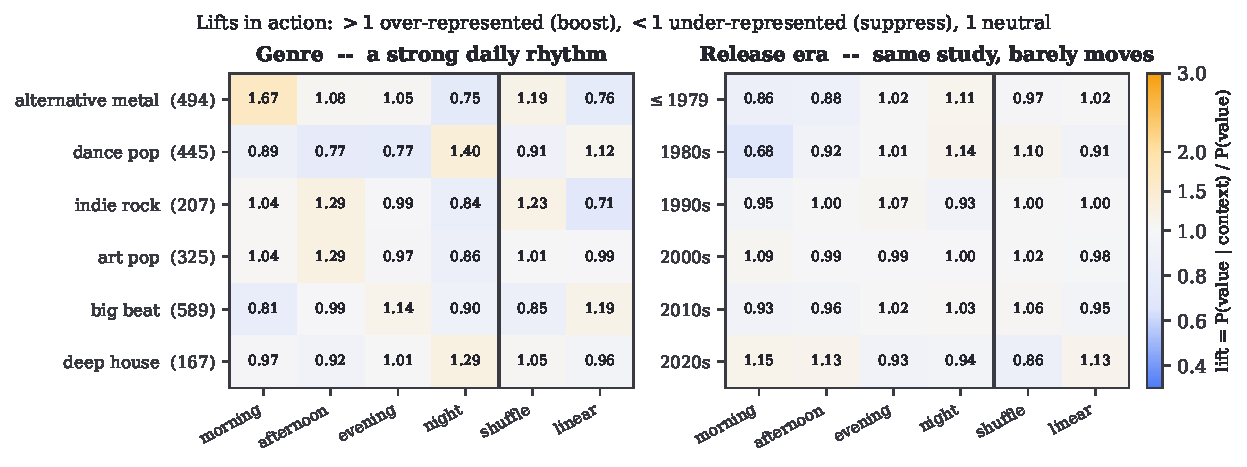
\includegraphics[width=\linewidth]{figures/fig_lifts.pdf}
\caption{Real lifts from the listening log, computed with one definition for both panels (track
counts in parentheses). Orange $=$ over-represented in that context (boost), blue $=$
under-represented (suppress), near-white $=$ neutral ($\approx 1$); the rule separates time-of-day
from shuffle state. \textbf{Left:} genre shows a strong daily rhythm. \textbf{Right:} release era,
run through the same pipeline, barely departs from neutral --- the rhythm is about genre, not era.}
\label{fig:lifts}
\end{figure}

\begin{figure}[H]\centering
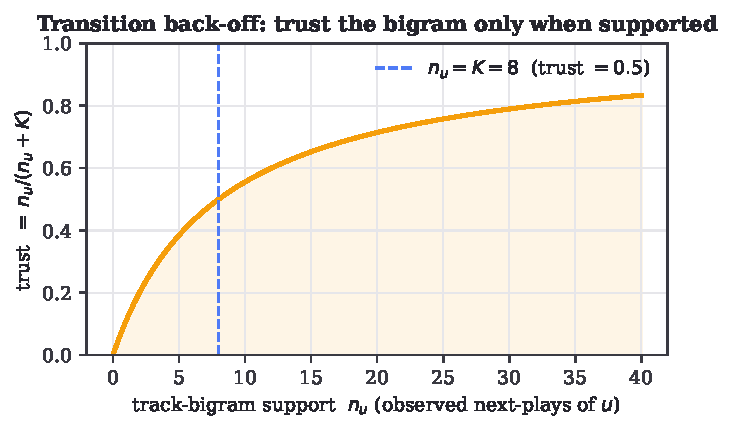
\includegraphics[width=0.58\linewidth]{figures/fig_backoff.pdf}
\caption{Back-off trust $\tau=n_u/(n_u+8)$, where the support $n_u$ is how many recorded successors
track $u$ has. Below $K=8$ observed next-plays the model leans on the
artist/genre back-off; above it, it trusts the track bigram. Both \code{affinity} and
\code{context\_fit} are min--max normalized across each expansion's candidates before entering the
A\textsuperscript{*} cost, so only \emph{relative} preference matters locally.}
\label{fig:transit}
\end{figure}

%====================================================================
\section{The $k$-nearest-neighbor graph}
\label{sec:knn}

A\textsuperscript{*} needs a sparse graph, not all-pairs distances. Offline, each track is connected
to its $k=20$ nearest neighbors by cosine distance; edges are made \textbf{symmetric} (if $A$ is near
$B$, $B$ links $A$) and sorted ascending. The graph (indices {+} distances) is baked into
\file{corpus.bin}, so at request time edge distances are a table lookup --- no vector math for graph
moves. Symmetry also widens the candidate pool that \code{densify} (\S\ref{sec:astar}) draws from.

\begin{figure}[H]\centering
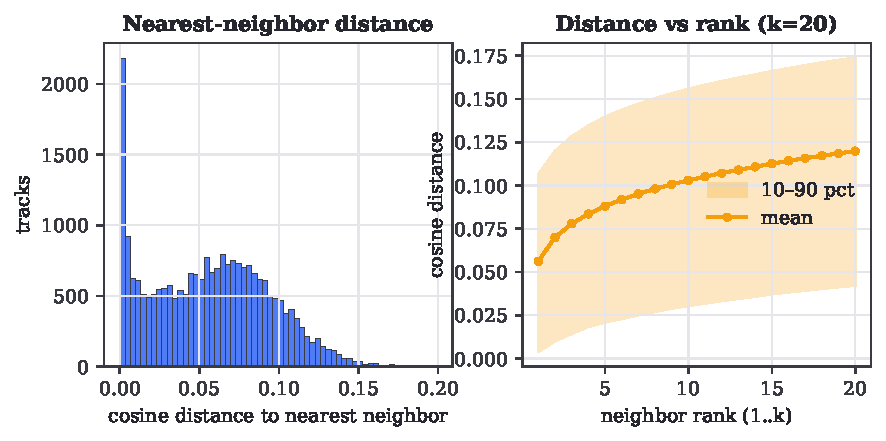
\includegraphics[width=\linewidth]{figures/fig_knn.pdf}
\caption{The real neighbor graph in \file{corpus.bin}. Left: distribution of the nearest-neighbor
cosine distance over all 23{,}529 tracks. Right: mean (and 10--90 percentile band) of cosine distance
versus neighbor rank $1\ldots20$ --- the local manifold density the search traverses.}
\label{fig:knn}
\end{figure}

%====================================================================
\section{Pathfinding: A\textsuperscript{*} with densify}
\label{sec:astar}

\textbf{The search.} Pathfinder runs A\textsuperscript{*} on the $k$-NN graph
(\file{worker-core/src/pathfind.rs}, a faithful port of \file{pathfinder/search.py}). The heuristic is
the cosine distance straight to the goal; the per-hop cost blends five interpretable, weighted terms:
\[
\text{step}(u\!\to\!v) = \underbrace{W_{\text{D}}\,d(u,v)}_{1.0}
+ \underbrace{W_{\text{F}}(1-\code{fit}_v)}_{0.5}
+ \underbrace{W_{\text{V}}\,[g_v\!\neq\!g_u]\,\gamma}_{0.5,\ \gamma=0.15}
+ \underbrace{W_{\text{T}}(1-\widetilde{\text{aff}})}_{0.6}
+ \underbrace{W_{\text{C}}(1-\widetilde{\text{ctx}})}_{0.4},
\]
where $\widetilde{(\cdot)}$ are the per-expansion min--max normalized transition and context scores.
Hard constraints forbid repeats, $>2$ consecutive same-artist tracks, and any artist exceeding
$\lceil L/4\rceil$ of an $L$-track route. If the found path is shorter than the requested length,
\code{densify} greedily inserts the best-scoring intermediate track into the widest remaining gap.

\begin{figure}[H]\centering
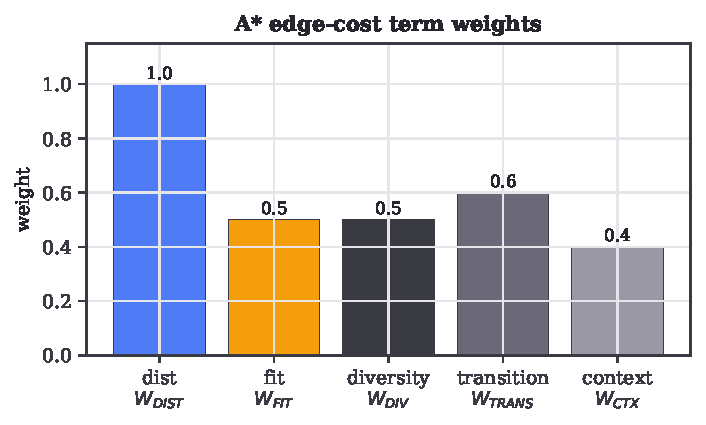
\includegraphics[width=0.6\linewidth]{figures/fig_cost_weights.pdf}
\caption{The five A\textsuperscript{*} edge-cost weights (\file{pathfinder/config.py}). Distance
dominates; transition history ($0.6$) outweighs time-of-day context ($0.4$); fit and genre-diversity
are equal soft terms.}
\label{fig:weights}
\end{figure}

\textbf{The CPU budget shapes the algorithm.} A faithful port is not enough: on the Free plan a
far-apart pair can blow the ${\sim}10$\,ms slice. The WASM core therefore caps the search at
\code{MAX\_EXPANSIONS = 45{,}000} and returns a clean ``no path'' (404) rather than being killed
mid-search (503). This is a deployment constraint leaking into algorithm design, not a modeling
choice.

\subsection{Response surfaces of the cost weights}
\label{sec:astarsweep}

The five weights are hand-set constants. To show how the \emph{found path} responds to them, we
re-ran the actual search (numpy port over the real \file{corpus.bin}\,/\,\file{transitions.json}) on
three fixed routes across two weight grids (Figure~\ref{fig:astarsweep}). These are
\emph{response surfaces of a deterministic search}, not trained-model error.

\begin{figure}[H]\centering
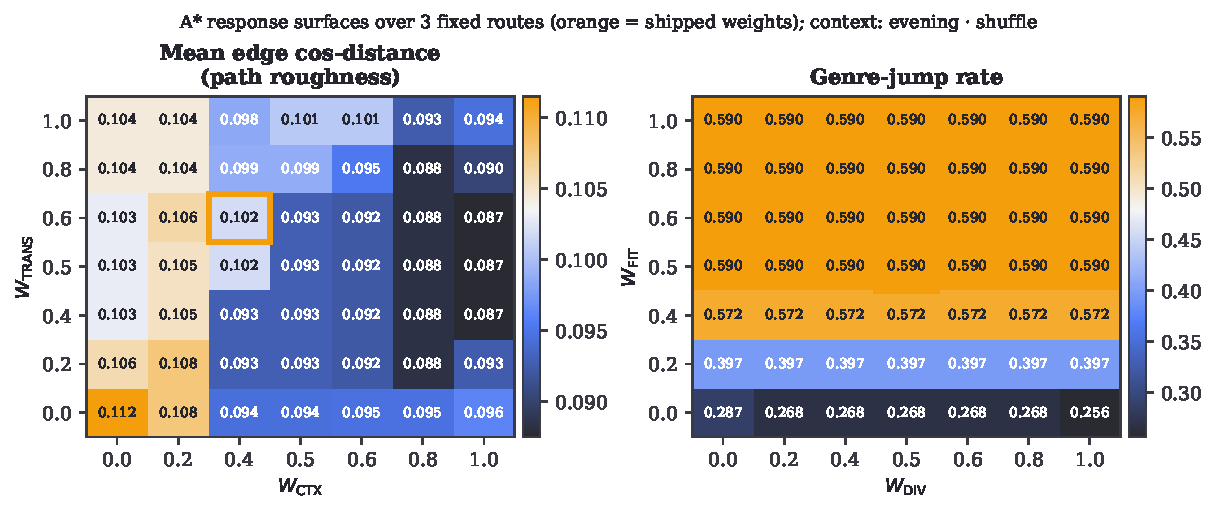
\includegraphics[width=\linewidth]{figures/fig_astar_sweep.pdf}
\caption{A\textsuperscript{*} response surfaces over the real corpus (orange = shipped weights).
\textbf{Left:} raising $W_{\text{CTX}}$ (and $W_{\text{TRANS}}$) yields measurably \emph{smoother}
paths (lower mean edge distance). \textbf{Right:} genre-jump rate climbs with $W_{\text{FIT}}$
(chasing high-fit tracks pulls across genres) but is nearly \emph{flat} in $W_{\text{DIV}}$ --- the
genre penalty $0.15\,W_{\text{DIV}}$ is too small to redirect these routes, confirming it is a gentle
soft constraint. Search capped at 15{,}000 expansions for tractability in Python.}
\label{fig:astarsweep}
\end{figure}

%====================================================================
\section{The 3D view: PCA by power iteration}
\label{sec:pca}

For rendering, the path and its neighborhood ``cloud'' are projected from 64-d to 3-d per request
(\file{worker-core/src/pca.rs}). To avoid a dense SVD dependency in WASM, the top-3 covariance
eigenvectors are found by \textbf{power iteration with deflation} --- cheap, since the covariance is
only $64\times64$ over ${\sim}100$ points --- then scaled by the 90th-percentile radius to $\pm8$.
Those axes capture most of the local variance (Figure~\ref{fig:pcavar}).

\begin{figure}[H]\centering
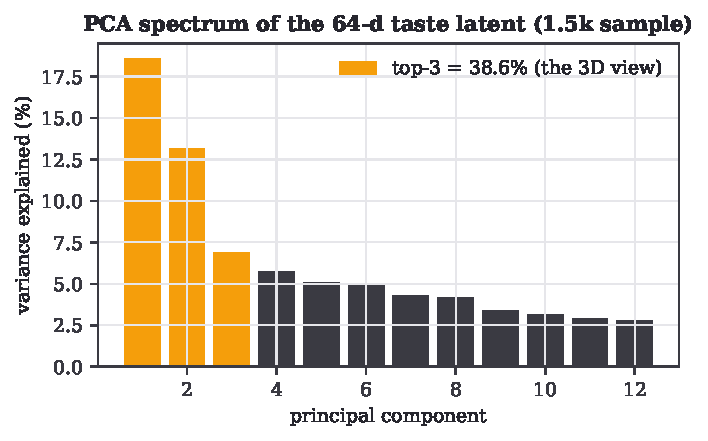
\includegraphics[width=0.55\linewidth]{figures/fig_pca_var.pdf}
\caption{Variance spectrum of the 64-d latent (1{,}500-track sample); the top-3 axes (orange) used
by the 3D view capture a large share, so the projection faithfully summarizes local structure.}
\label{fig:pcavar}
\end{figure}

%====================================================================
\section{Validation and parity}
\label{sec:parity}

Because the request-time core is a Rust rewrite of Python references, correctness is enforced by
tests, not assumed. A \textbf{parity test} (\file{worker-core/tests/parity.rs}) checks the Rust
A\textsuperscript{*} against \file{search.py} on corpus routes: identical endpoints/length, all
constraints satisfied, Rust cost $\le 1.6\times$ Python cost $+\,0.1$, and $\ge 85\%$ node identity on
at least one case. The tolerance is deliberate --- heuristic search legitimately yields alternate
near-optimal paths under float reordering, so exact byte-match is the wrong bar. A second test
round-trips the projector binary to guard the \file{PFP1} format. Significance of \emph{model}
differences is judged against the measured noise band $\sigma_{\text{AUC}}=0.0063$
(Figure~\ref{fig:bakeoff}), not eyeballed.

%====================================================================
\section{Lessons and rationale}
\label{sec:lessons}

\begin{itemize}[leftmargin=1.4em,itemsep=3pt]
\item \textbf{Identity $>$ architecture} (documented). One-hot artist/genre features in trees beat
every dense embedding and every margin model; the Song-AE latent, useful as \emph{geometry}, dilutes
as a \emph{feature}. Scan feature/dataset axes before tuning models.
\item \textbf{Tuning $<$ noise, here} (this report). The deferred depth/lr/n\_est scan
(Figure~\ref{fig:xgbsweep}) moves AUC by less than the 3-seed band --- evidence the deferral was
correct and the champion defaults are adequate.
\item \textbf{Honest metrics} (documented). The pivot to rotation{+}AUC/logloss followed concrete
failures of MAE on a binary target (the $\varepsilon$-tube artifact, blend-weight collapse).
\item \textbf{Frozen outputs beat live inference} (architecture). Baking model outputs into a snapshot
is what lets seven models serve from a 10\,ms Worker; the cost is a rebuild-to-refresh cycle.
\item \textbf{Two latent uses, one space} (architecture). The projector exists only because a Worker
cannot run the real encoder; it is a deliberately lossy translator, backed by a snap-to-anchor step.
\end{itemize}

\appendix
%====================================================================
\section{Snapshot binary formats}
\label{app:formats}

\begin{table}[H]\centering\small
\caption{\file{corpus.bin} (\code{PFC1}) and \file{projector.bin} (\code{PFP1}) layouts, little-endian.
$n{=}23{,}529$, $\dim{=}64$, $k{=}20$; projector $\text{in}{=}1179$, $h{=}256$, $\text{out}{=}64$.}
\label{tab:formats}
\begin{tabular}{@{}llll@{}}
\toprule
\multicolumn{2}{c}{\code{PFC1} corpus.bin} & \multicolumn{2}{c}{\code{PFP1} projector.bin}\\
\cmidrule(r){1-2}\cmidrule(l){3-4}
field & type & field & type \\
\midrule
magic\,/\,ver\,/\,$n$\,/\,dim\,/\,$k$ & \code{u32}$\times$5 & magic\,/\,ver\,/\,in\,/\,$h$\,/\,out\,/\,text & \code{u32}$\times$6 \\
ids & \code{u64}$[n]$ & $W_1$ & \code{f32}$[h{\cdot}\text{in}]$ \\
vecs (L2-norm) & \code{f32}$[n{\cdot}\dim]$ & $b_1$ & \code{f32}$[h]$ \\
fit & \code{f32}$[n]$ & $W_2$ & \code{f32}$[\text{out}{\cdot}h]$ \\
nbr\_idx & \code{u32}$[n{\cdot}k]$ & $b_2$ & \code{f32}$[\text{out}]$ \\
nbr\_dist & \code{f32}$[n{\cdot}k]$ & cfg\_len & \code{u32} \\
meta\_len {+} JSON & \code{u32}{+}bytes & cfg (stats, vocab) & JSON \\
\bottomrule
\end{tabular}
\end{table}

\section{Constants}
\label{app:constants}

\begin{table}[H]\centering\small
\begin{tabular}{@{}llll@{}}
\toprule
A\textsuperscript{*} cost & value & transition / search & value \\
\midrule
$W_{\text{DIST}}$ & 1.0 & $K$ (back-off) & 8.0 \\
$W_{\text{FIT}}$ & 0.5 & artist / genre weight & 0.6 / 0.4 \\
$W_{\text{DIV}}$ & 0.5 & max consecutive artist & 2 \\
$W_{\text{TRANS}}$ & 0.6 & artist share divisor & 4.0 \\
$W_{\text{CTX}}$ & 0.4 & MAX\_EXPANSIONS & 45{,}000 \\
genre-jump $\gamma$ & 0.15 & $k$-NN $k$ & 20 \\
\bottomrule
\end{tabular}
\caption{Cost weights and constants (\file{pathfinder/config.py}, \file{transit.rs}).}
\end{table}

\begin{table}[H]\centering\small
\begin{tabular}{@{}lll@{}}
\toprule
XGBoost champion & value & data \\
\midrule
n\_estimators / max\_depth & 500 / 6 & dataset \code{ds-...-141622-p1-s42} \\
learning\_rate & 0.05 & 115 cols, 9805 train / 2451 test \\
subsample / colsample & 0.8 / 0.8 & AUC 0.7429, logloss 0.5883 \\
reg\_lambda / seed & 1.0 / 42 & $\sigma_{\text{AUC}}=0.0063$ (3 seeds) \\
\bottomrule
\end{tabular}
\caption{Rotation classifier (\file{predictors/xgboost-classifier/train.py}; metrics from
\file{data/runs/}).}
\end{table}

\section{Undocumented / open questions}
\label{app:open}

For honesty, what the source artifacts do \emph{not} establish: (i) why 64 latent dims, or any
ablation of Song-AE depth/width; (ii) XGBoost tree-level tuning provenance --- the grid in
\S\ref{sec:xgbsweep} was run by us, not recovered; (iii) smoothing/thresholds in the transition-table
construction beyond the satisfaction weights and support shrinkage; (iv) provenance of the
A\textsuperscript{*} weight values --- they are constants with no recorded tuning study (our
Figure~\ref{fig:astarsweep} probes behavior, not optimality); (v) end-to-end request latency and
cold-start path behavior on deployed hardware, which \file{WORKLOG.md} notes is untested.

\section{Reproducibility}
\label{app:repro}

Every figure regenerates from the repository. Sweeps (write \file{docs/sweeps/*.json}):
\begin{quote}\small\ttfamily
predictors/.venv/bin/python docs/sweeps/run\_xgb\_sweep.py\\
\$ANACONDA/bin/python docs/sweeps/run\_astar\_sweep.py\\
\$ANACONDA/bin/python docs/sweeps/load\_runs.py
\end{quote}
Figures and document:
\begin{quote}\small\ttfamily
\$ANACONDA/bin/python docs/make\_figures.py\\
cd docs \&\& tectonic models.tex
\end{quote}

\end{document}
